\chapter{PENGUJIAN}
\label{chap:chap4_pengujian}
\vspace{1ex}

\section*{}
Inti dari BAB \ref{chap:chap4_pengujian} pada penelitian adalah pengujian dengan berbagai parameter untuk \textit{stats} pemain dan musuh. Seperti halnya \textit{stats} pemain dan musuh pada permainan dengan genre \textit{turn-based} dan \textit{action} RPG.
\vspace{1ex}

\section{Pengujian dalam Pembuatan \textit{Stats} Pemain pada Permainan dengan Genre \textit{Turn-based} RPG}
\label{sec:sec4_pengujian_turn-based_player}
\vspace{1ex}

Pada bagian ini setiap langkah yang akan diuji sudah dijelaskan pada Sub-bab \ref{sec:sec3_player_stats}, dimana pada bagian ini membahas tentang pembuatan \textit{stats} pemain untuk permaian dengan genre \textit{turn-based} RPG. Melalui berbagai proses seperti yang dijelaskan pada Sub-bab \ref{sec:sec3_player_stats}, maka pada beberapa Sub-bab dibawah ini adalah langkah-langkah dalam proses pengujiannya.
\vspace{1ex}

\subsection{Distibusi Level, HP, dan MP Pemain}
\label{sec:sub_sec4_eval_dist_hp_mp_level}
\vspace{1ex}

Seperti yang sudah dijelaskan pada Sub-bab \ref{sec:sub_sec3_enemy_hp_mp_stats}, dimana pada bagian ini membahas tentang pembuatan level, HP dan MP pemain untuk permaian dengan genre \textit{turn-based} RPG. Berikut adalah hasil dari prosess pembuatan Level, HP, dan MP yang dipeeroleh dari perhitungan pada persamaan \ref{eq:hp_player} dan \ref{eq:mp_player} dengan data masukan pada Tabel \ref{tb:player_input_variable} yang kemudian menghasilkan data seperti yang ditunjukkan pada Tabel \ref{tb:player_hp_mp}. 

\begin{longtable}{|l|l|l|}
	\caption{Hasil Perhitungan HP dan MP}
	\label{tb:player_hp_mp}\\
	\hline
	\rowcolor[HTML]{C0C0C0} 
	\textbf{Levels} & \textbf{HP} & \textbf{MP} \\ \hline
	1 & 159 & 89 \\ \hline
	2 & 163 & 93 \\ \hline
	3 & 167 & 97 \\ \hline
	4 & 171 & 101 \\ \hline
	5 & 175 & 105 \\ \hline
	6 & 179 & 109 \\ \hline
	7 & 183 & 113 \\ \hline
	... & ... & ... \\ \hline
	\textbf{100} & \textbf{555} & \textbf{485} \\ \hline
\end{longtable}
\vspace{1ex}

Hasil perhitungan tersebut terlihat membentuk pola linier, yang mana nilai HP dan MP terus naik secara konstan ke atas sesuai dengan kenaikan levelnya seperti yang direpresentasikan pada Gambar \ref{fig:hp_player} dan Gambar \ref{fig:mp_player}.

\begin{figure} [!h] \centering
	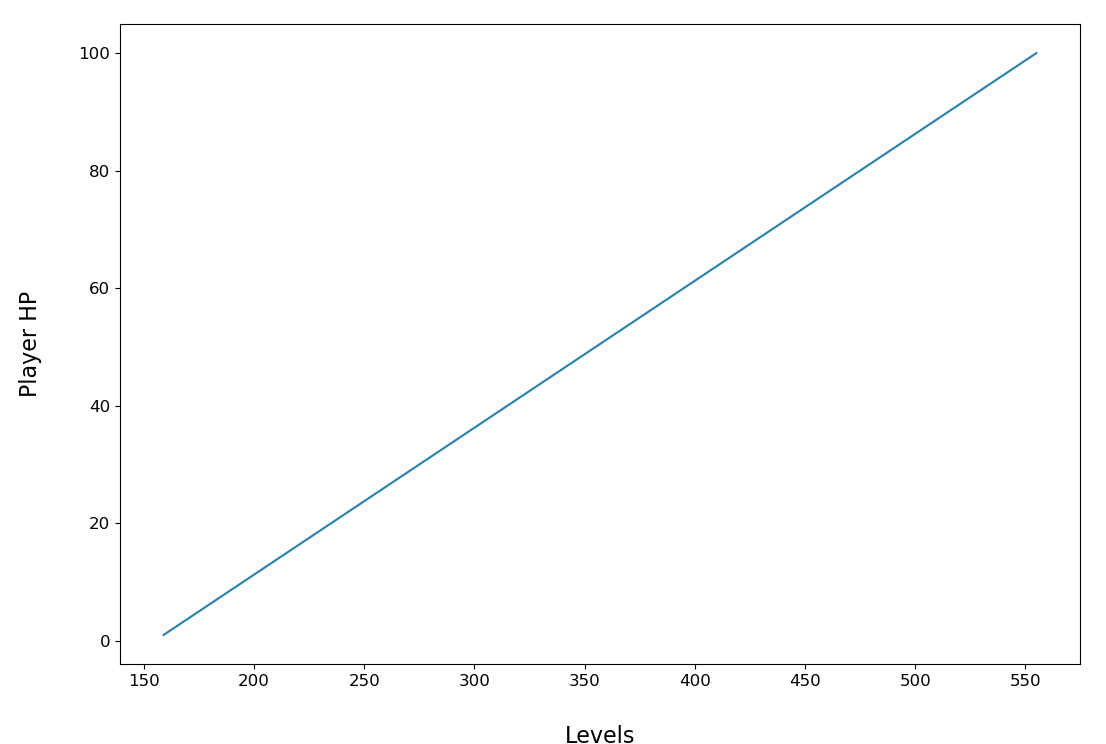
\includegraphics[scale=0.45]{img/PlayerHpDistrib.png}
	\caption{Kenaikan HP setiap levelnya.}
	\label{fig:hp_player}
\end{figure}

Jika melihat Gambar \ref{fig:hp_player} dengan jumlah HP dari pemain yang terus naik mengikuti pola yang dihasilkan pada Tabel \ref{tb:player_hp_mp}, yang mana nilai tersebut diperoleh dari inisiasi variabel pada Tabel \ref{tb:player_input_variable} yaitu \textit{Max Level}, \textit{Start} HP dan \textit{Next} HP. Variabel-variabel tersebut dihitung dengan menggunakan persamaan \ref{eq:hp_player} agar membentuk pola kenaikan HP setiap levelnya seperti yang ditunjukan pada Gambar \ref{fig:hp_player}. Sama seperti pada Gambar \ref{fig:hp_player}, pada Gambar \ref{fig:mp_player} dengan jumlah MP dari pemain yang terus naik mengikuti pola yang dihasilkan pada Tabel \ref{tb:player_hp_mp}, yang mana nilai tersebut diperoleh dari inisiasi variabel pada Tabel \ref{tb:player_input_variable} yaitu \textit{Max Level}, \textit{Start} MP dan \textit{Next} MP. Kemudian variabel-variabel tersebut dihitung dengan menggunakan persamaan \ref{eq:mp_player} agar membentuk pola kenaikan MP setiap levelnya seperti yang ditunjukan pada Gambar \ref{fig:mp_player}.

\begin{figure} [!h] \centering
	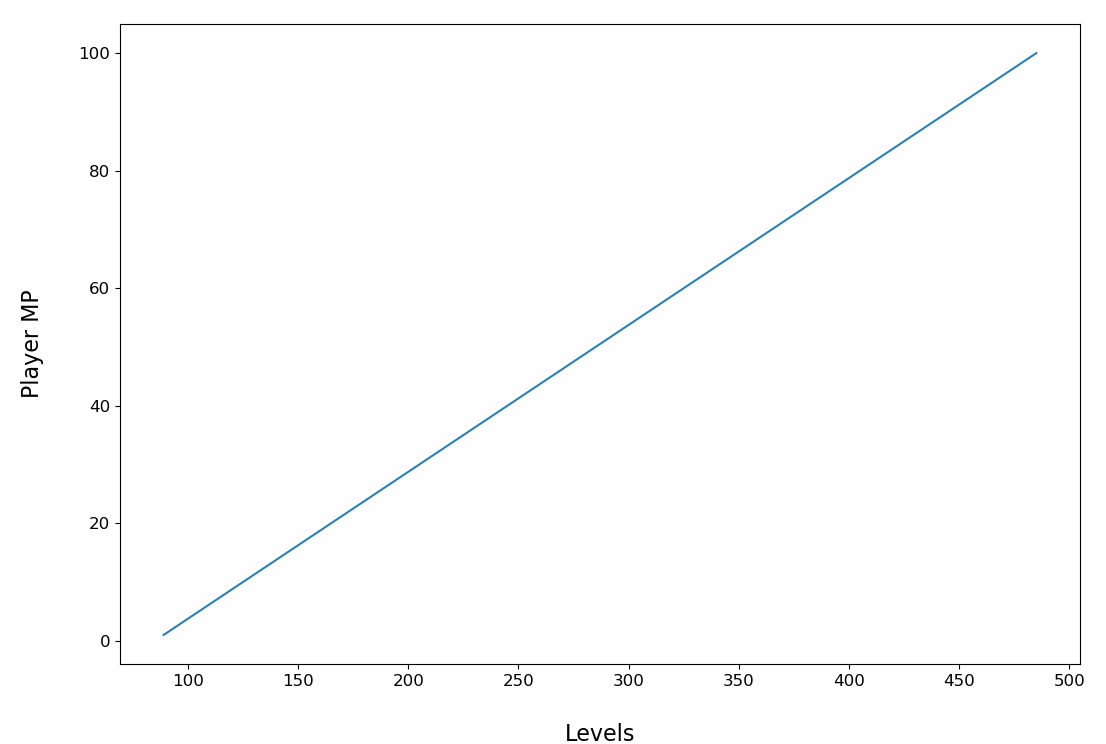
\includegraphics[scale=0.45]{img/PlayerMpDistrib.png}
	\caption{Kenaikan MP setiap levelnya.}
	\label{fig:mp_player}
\end{figure}
\vspace{1ex}

\subsection{Distibusi Stats Pemain}
\label{sec:sub_sec4_pengujian_player_stats}
\vspace{1ex}

Pada bagian ini setiap langkah yang akan diuji sudah dijelaskan pada Sub-bab \ref{sec:sub_sec3_stat_pemain}, dimana pada bagian ini membahas tentang pembuatan \textit{stats} pemain untuk permaian dengan genre \textit{turn-based} RPG. Melalui berbagai proses seperti yang dijelaskan pada Sub-bab \ref{sec:sub_sec3_stat_pemain}, melalui persamaan \ref{eq:KNN_bayes_player_stats} dan beberapa persamaan yang digunakan sebelumnya pada Sub-bab \ref{sec:sub_sec3_stat_pemain} dihasilkan data seperti yang ditunjukan pada Tabel \ref{tb:player_battle_stats}, dan bila divisualisasikan hasilnya akan tampak seperti pada Gambar \ref{fig:stats_player}.

\begin{longtable}{|l|l|l|l|l|l|}
	\caption{Sampel hasil perhitungan dan distribusi stats dengan $k-$NN}
	\label{tb:player_battle_stats}\\
	\hline
	\rowcolor[HTML]{C0C0C0} 
	\textbf{Levels} & \textbf{Strength} & \textbf{Magic} & \textbf{Endurance} & \textbf{Speed} & \textbf{Luck} \\ \hline
	1 & 1 & 2 & 0 & 0 & 1 \\ \hline
	2 & 0 & 2 & 0 & 2 & 0 \\ \hline
	3 & 1 & 0 & 0 & 0 & 0 \\ \hline
	4 & 1 & 1 & 0 & 0 & 0 \\ \hline
	5 & 1 & 1 & 0 & 0 & 0 \\ \hline
	6 & 1 & 1 & 0 & 2 & 1 \\ \hline
	7 & 0 & 0 & 0 & 0 & 1 \\ \hline
	8 & 1 & 0 & 0 & 0 & 0 \\ \hline
	... & ... & ... & ... & ... & ... \\ \hline
	\textbf{100} & \textbf{1} & \textbf{0} & \textbf{0} & \textbf{0} & \textbf{0} \\ \hline
\end{longtable}

\begin{figure} [!h] \centering
	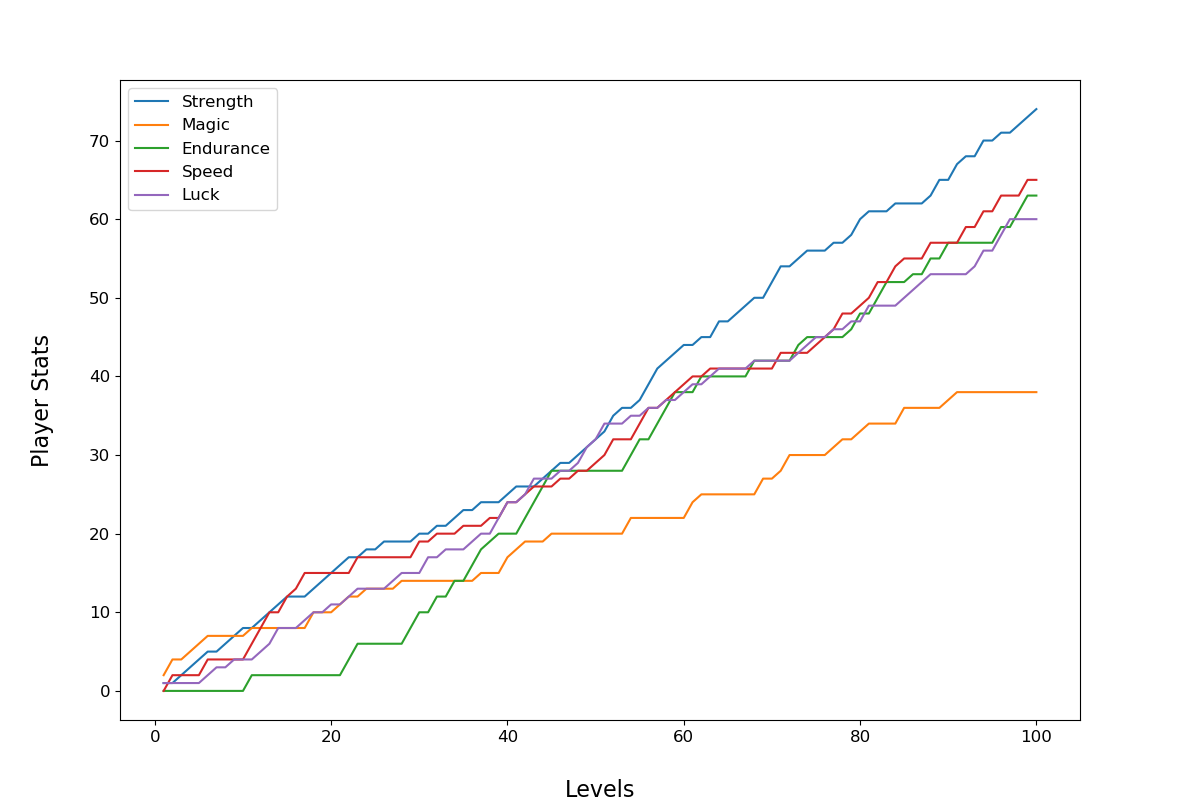
\includegraphics[scale=0.50]{img/PlayerStatsDistrib.png}
	\caption{Kenaikan stats pemain setiap levelnya.}
	\label{fig:stats_player}
\end{figure}

Pada Tabel \ref{tb:player_battle_stats} adalah data \textit{stats} dari pemain yang dihasilakn melalui penambahan nilai pada \textit{stats} secara acak pada setiap \textit{stats}. Seperti yang dijelaskan pada persaamaan \ref{eq:nbayes_class}, \ref{eq:KNN_distance_stats}, dan persamaan \ref{eq:KNN_bayes_player_stats} saat nilai \textit{stats} di tambahkan secara acak dari 1 sampai dengan 2 pada level yang berjarak antara 1 sampai dengan 100. Selanjutnya representasi dari hasil penambahan \textit{stats} tersebut yang ditunjukan melalui Gambar \ref{fig:stats_player} yang mana nilai dari setiap \textit{stats} terus naik sesuai dengan level pemain yang juga terus naik. 
\vspace{1ex}

\section{Pengujian dalam Pembuatan \textit{Stats} Musuh pada Permainan dengan Genre \textit{Turn-based} RPG}
\label{sec:sec4_pengujian_turn-based_enemy}
\vspace{1ex}

Pada bagian ini setiap langkah yang akan diuji sudah dijelaskan pada Sub-bab \ref{sec:sec3_enemy_stats}, dimana pada bagian ini membahas tentang pembuatan \textit{stats} musuh untuk permaian dengan genre \textit{turn-based} RPG. Melalui berbagai proses seperti yang dijelaskan pada Sub-bab \ref{sec:sec3_player_stats}, maka pada beberapa Sub-bab dibawah ini adalah langkah-langkah dalam proses pengujiannya.
\vspace{1ex}

\section{Pengujian dalam Pembuatan \textit{Stat} Pemain untuk Permainan dengan Genre \textit{Action} RPG}
\label{sec:sec4_pengujian_player}
\vspace{1ex}

Sama seperti pengujian yang dilakukan pada Sub-bab \ref{sec:sec4_pengujian_turn-based_player} yang mana langkahnya sudah dijelaskan pada Sub-bab \ref{sec:sec3_player_stats}, hanya saja pada bagian ini membahas tentang pembuatan dan penyesuaian \textit{stats} pada permaian untuk genre \textit{action} RPG. Melalui berbagai proses seperti yang dijelaskan pada Sub-bab \ref{sec:sec4_pengujian_turn-based_player} tentang \textit{turn-based} RPG, hanya saja pada bagian ini tidak memerlukan elemen yang menggambarkan kelemahan dari karakter pemain yang mana hal inilah yang disebut dengan penyesuaian. Melalui beberapa Sub-bab dibawah ini adalah langkah-langkah dalam proses pengujiannya.
\vspace{1ex}

\section{Pengujian dalam Pembuatan \textit{Stas} Musuh untuk Permainan dengan Genre \textit{Action} RPG}
\label{sec:sec4_pengujian_enemy}
\vspace{1ex}

Sama seperti pengujian yang dilakukan pada Sub-bab \ref{sec:sec4_pengujian_turn-based_player} yang mana langkahnya sudah dijelaskan pada Sub-bab \ref{sec:sec3_player_stats}, hanya saja pada bagian ini membahas tentang pembuatan dan penyesuaian \textit{stats} pada permaian untuk genre \textit{action} RPG. Melalui berbagai proses seperti yang dijelaskan pada Sub-bab \ref{sec:sec4_pengujian_turn-based_player} tentang \textit{turn-based} RPG, hanya saja pada bagian ini tidak memerlukan elemen yang menggambarkan kelemahan dari karakter pemain yang mana hal inilah yang disebut dengan penyesuaian. Melalui beberapa Sub-bab dibawah ini adalah langkah-langkah dalam proses pengujiannya.